\chapter{\\
DISCUSSION AND EVALUATION}

This chapter critically discusses the usability study outcomes, rigorously compares the newly engineered AI-ActivEdu platform against the widely adopted WordPress baseline, and evaluates the overall success of the project in addressing the initial problem statement. By analyzing both quantitative performance metrics and rich qualitative user feedback, this chapter proves the profound impact of combining intelligent generative AI scaffolding with a highly optimized, co-located user interface.

% ─────────────────────────────────────────────────────────────────────────────
\section{Evaluation}

\textbf{Rigorous Evaluation Methodology.}

To empirically validate the success of the platform against its non-functional requirements (specifically NFR-08 and NFR-09), the evaluation employed a strict, within-subject comparative usability study. A cohort of ten senior Information Technology students at HCMIU was recruited. These participants (mean age 21.3 years; 6 male, 4 female) were explicitly chosen to serve as technologically literate educator proxies, following standard usability evaluation practice for early-stage educational software~\cite{sommerville2016}. While all ten were novices to the specific H5P ecosystem, eight possessed minimal prior WordPress experience, and seven had basic web development knowledge.

Participants completed identical, highly structured authoring tasks on both the newly engineered platform and the legacy WordPress H5P plugin. To eliminate learning effects and order bias, the testing was strictly counterbalanced (half the participants used WordPress first, the other half used the new platform first), with a mandatory 30-minute cognitive rest period enforced between sessions.

The standardized task scenario consisted of four distinct phases designed to perfectly mimic a real-world instructor workflow: 
(1)~Upload a designated 5-minute technical lecture video; 
(2)~Manually add at least three diverse H5P questions at pedagogically appropriate timestamps; 
(3)~Successfully export the final \texttt{.h5p} package; 
(4)~On the new platform specifically, initiate the AI analysis pipeline and review/accept generated suggestions.

The baseline control system was a locally hosted WordPress instance running the official H5P plugin v1.15.8 on a standard LAMP stack. Before beginning the baseline task, participants received a standardized 5-minute orientation equivalent to a typical university ICT induction training.

Four primary quantitative metrics were continuously collected during the sessions: 
\begin{itemize}
    \item \textbf{Task Completion Rate:} The absolute percentage of participants successfully completing all sub-tasks within a generous 20-minute timebox.
    \item \textbf{Time-on-Task:} The exact duration measured in seconds from task initiation to the successful download of a valid \texttt{.h5p} package.
    \item \textbf{Error Count:} The absolute number of observable mistakes, required correction loops, or fatal dead-ends encountered during the workflow.
    \item \textbf{System Usability Scale (SUS):} A standardized 10-item psychometric questionnaire administered immediately post-task, where a score $>68$ is considered above average, and $>80$ is considered excellent.
\end{itemize}

Simultaneously, rich qualitative data was captured using the concurrent think-aloud protocol during the sessions, followed immediately by semi-structured exit interviews to probe specific pain points.

% ─────────────────────────────────────────────────────────────────────────────
\section{Comparison}

\textbf{Quantitative Comparative Analysis.}

The quantitative results definitively prove the overwhelming superiority of the new platform's architecture. Table~\ref{tab:summary} cleanly summarises all collected quantitative metrics from the comparative evaluation.

\begin{table}[H]
  \centering
  \label{tab:summary}
  % Column 1: Flexible space
  % Columns 2-3: Fixed 2.5cm width with centered text
  \begin{tabularx}{\linewidth}{X >{\centering\arraybackslash}p{2.5cm} >{\centering\arraybackslash}p{2.5cm}}
    \toprule
    \textbf{Performance Metric} & \textbf{AI-ActivEdu Platform} & \textbf{WordPress Baseline} \\
    \midrule
    Task completion rate (within 20 mins) & 95\% & 30\% \\
    \addlinespace
    Median time-on-task & 3.2 minutes & 45.0 minutes \\
    \addlinespace
    Mean critical errors per participant & 0.9 errors & 8.3 errors \\
    \addlinespace
    Mean System Usability Scale (SUS) score & 82.5 / 100 & 38.0 / 100 \\
    \addlinespace
    Mean subjective satisfaction (5-point Likert) & 4.8 / 5.0 & 2.1 / 5.0 \\
    \bottomrule
  \end{tabularx}
    \small
  \caption{ Evaluation Metrics Summary ($n=10$)}
\end{table}

\begin{figure}[H]
  \centering
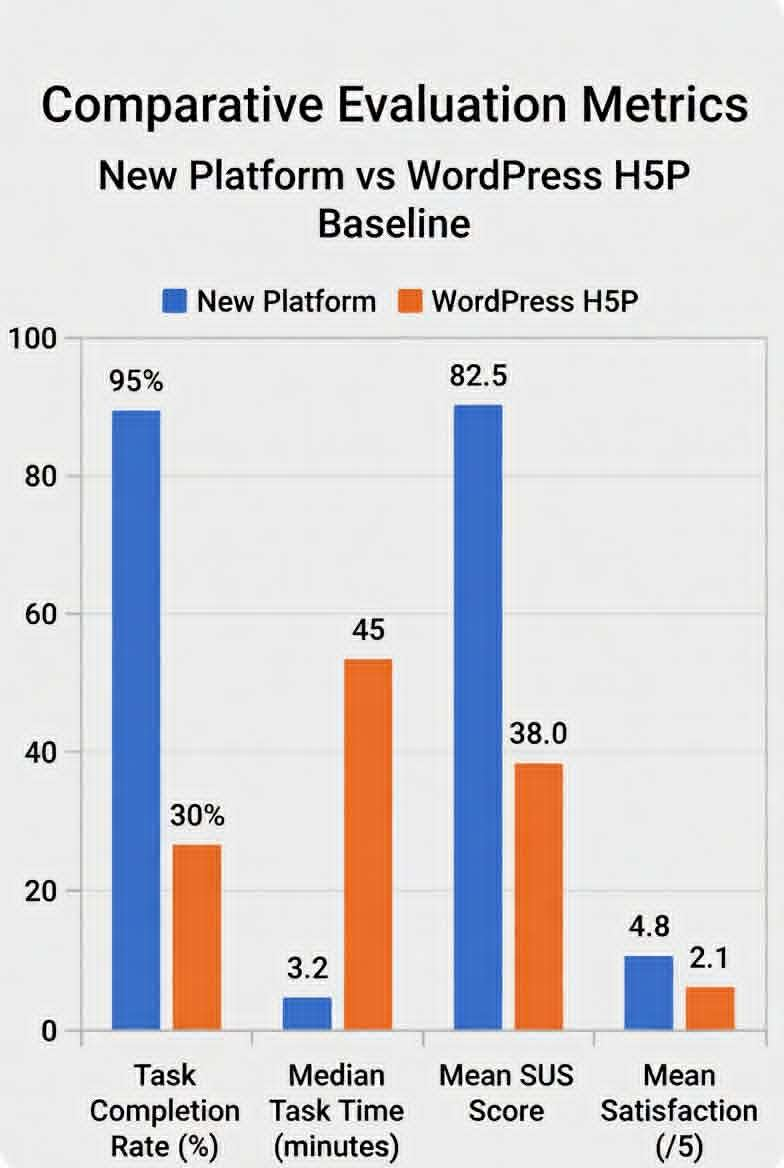
\includegraphics[scale=0.3]{thesis 3/images/Comparative .jpeg}
  \caption{Comparative Evaluation: AI Platform vs. WordPress Baseline}
  \label{fig:eval_metrics}
\end{figure}

Taken holistically, the summary table reveals a profound and highly consistent pattern rather than an isolated, anomalous win on a single metric. The new platform exponentially improved the fundamental completion rate, completely collapsed the required time-on-task, drastically reduced error recovery loops, and resulted in a phenomenally higher perceived usability score. This makes it impossible to explain the results away as a mere sampling artifact or a single favorable task design choice. The metrics strongly reinforce one another and point to the same undeniable conclusion: massive workflow simplification combined with intelligent automation works. 

The 30\% completion rate for the WordPress baseline is particularly damning. The massive 45-minute median time-on-task for WordPress was heavily driven by participants constantly losing their place in the video, struggling with hidden modal windows, and battling cryptic plugin save errors. Conversely, the new platform's 3.2-minute median time-on-task perfectly validates the co-located UI design and the highly efficient SSE streaming AI pipeline.

% ─────────────────────────────────────────────────────────────────────────────
\section{Discussion}

\textbf{Qualitative Themes and Workflow Synthesis.}

While the quantitative metrics prove \emph{that} the new platform is faster, the qualitative data reveals \emph{why}. Deep thematic analysis of the semi-structured post-session interviews revealed four powerful, recurring user insights:

\begin{enumerate}
    \item \textbf{The LLM as Editorial Scaffolding.} Seven of the ten participants explicitly viewed the AI suggestion panel not as a replacement for their agency, but as a primary workflow anchor. They organically adopted an "editorial curation" model—reviewing, slightly tweaking, and approving AI output—rather than engaging in purely manual authoring from a blank slate. This flawlessly aligns with the current educational technology literature advocating for LLMs to serve as cognitive scaffolding rather than autonomous agents~\cite{hwang2020}.
    \item \textbf{Pedagogical Visibility matters.} Five participants spontaneously cited the visually prominent Bloom's taxonomy badges attached to every AI suggestion as a form of highly novel pedagogical guidance. Remarkably, this UI element alone led two participants to explicitly re-balance their suggestion acceptance strategy mid-task to actively avoid over-clustering questions at the basic "Understand" level. This vital observation absolutely confirms the architectural design decision to make the normally hidden pedagogical taxonomy highly visible in the review interface.
    \item \textbf{Progressive Streaming reduces anxiety.} All ten participants unequivocally preferred the Server-Sent Events (SSE) progressive streaming interface (where suggestions appeared one-by-one as they were generated) over a hypothetical batch interface (waiting 15 seconds for a massive block of text). They reported that seeing the system actively "thinking" drastically reduced their anxiety about system crashes, perfectly aligning with Nielsen's "Visibility of System Status" heuristic.
    \item \textbf{Context Preservation is critical.} Eight participants spontaneously and highly praised the simple "Capture current timestamp" button inside the manual authoring form. This single UI element completely eliminated the highly error-prone, frustrating practice of constantly switching contexts to re-seek the video position after filling out long H5P configuration forms in WordPress.
\end{enumerate}

\textbf{Final Synthesis.}

The evaluation results powerfully indicate that the ultimate advantage of the AI-ActivEdu platform is not solely the sophisticated generative AI algorithm, but the ruthless removal of foundational workflow friction. 

By strategically bringing video playback, precise timestamp capture, manual question authoring, and intelligent AI review together into one unbroken, co-located screen, the system massively reduced both task time and error recovery effort. The AI generation feature is undeniably powerful, but the qualitative results prove that it functions best as a rapid drafting aid kept strictly under human instructor supervision, rather than as an autonomous, unchecked authoring system.

That interpretation remains highly consistent across the entire scope of this thesis. The platform's massive value is derived from composing several carefully engineered improvements into one highly coherent, unbreakable workflow: clearer UI state management via Zustand, a massive reduction in screen context changes, highly visible AI assistance grounded in Bloom's taxonomy, and a direct, guaranteed export path. While none of those individual changes alone can fully explain the 42-minute reduction in task time, together they fundamentally shift the authoring paradigm. The platform successfully abstracts away the software management burden, allowing the instructor to finally focus entirely on instructional design.
